\section{The Diffie-Hellman key exchange}
Since public key cryptosystems are relatively slowly compared to private key ones, it is often more realistic to use them in conjunction with classical schemes, giving them the limited role of key exchange and agreement.

A major flaw of symmetric cryptosystems, in fact, is that key establishment must be done through secure means, and \textbf{information cannot directly be sent over the channel}. The two parts must have prior knowledge and trust of each other, and cannot publicly share information. 

This can be solved encrypting a symmetric key using a public key algorithm, so that after the decryption it can be used by both parts to encrypt and decrypt using the symmetric cipher. 

The first published proposal for a \textbf{key exchange based on public cryptography} is attributed to W. Diffie and M. E. Hellman, and was based on the discrete logarithm problem.

The process involves two individuals agreeing on an arbitrary starting number which does not have to be kept secret, while each one secretly chooses another value to keep to himself. Then, the secret is mixed with the public key, and the result is exchanged. 

Finally, the received output is once again combined with the other secret, giving the original message. If a third party listened to the exchange, it would only know the common number and the mixed one, with the inability to retrieve the original value in an efficient way.

Diffie-Hellman is not an encryption algorithm, but rather a \textit{protocol} defining the necessary series of step in order to achieve the exchange of encrypted information between two parties through asymmetrical cryptography. 

The basic idea behind the Diffie-Hellman Key Exchange (DHKE) is that exponentiation in $\mathbb{Z}^*_p$ with $p$ prime is a one-way function and the exponentiation is commutative, i.e.:
$$k = (a^x)^y \equiv (a^y)^x \mod p$$

The value $k$ is the joint secret which can be used as session key between the two parties. 

The set-up protocol consists of the following steps:
\begin{enumerate}
	\item Choose a large prime $p$;
	\item Choose an integer $\alpha \in \{2, 3, \dots, p - 2\}$, which ideally should be a generator;
	\item Publish $p$ and $\alpha$ (domain parameters).
\end{enumerate}

If Alice and Bob both know the public parameters $p$ and $\alpha$, they can generate a joint secret key $k$ with the DHKE protocol:

\begin{figure}[h]
	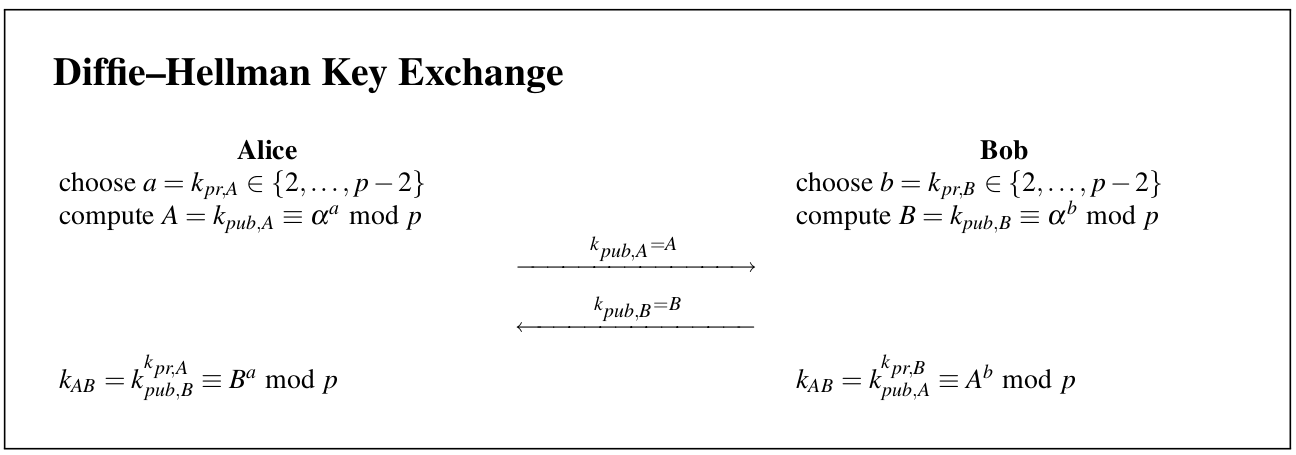
\includegraphics[scale=0.35]{DiffieHellmanPaar.png}
	\centering
\end{figure}

Enciphering and deciphering between Alice and Bob can now be performed by both parts:
$$k_{AB} = k^{k_{pr, A}}_{k_{pub, B}} \equiv B^a \mod p$$
$$k_{AB} = k^{k_{pr, B}}_{k_{pub, A}} \equiv A^b \mod p$$

The correctness of this protocol is simple to prove: 
\begin{itemize}
	\item Alice computes $B^a \equiv (\alpha^b)^a \equiv \alpha^{ab} \mod p$;
	\item Bob computes $A^b \equiv (\alpha^a)^b \equiv \alpha^{ab} \mod p$.
\end{itemize}
Now both of them share the session key $k_{AB} \equiv \alpha^{ab} \mod p$ which can be used to establish a secure connection for a symmetric algorithm. 

This protocol can also be extended with more than two parties: any number of users can take part in the exchange by performing more iterations of the algorithm and exchanging intermediate data.

\subsection{Security of Diffie-Hellman}
Basic Diffie-Hellman protocol is not secure against active attacks: messages can be either modified or falsely generated by a malicious third part, harming its security through a so called man-in-the-middle attack. 

However, if generators and finite groups are chosen carefully and large enough, the protocol is considered secure. 

Passive attacks. i.e.\ ones in which an attacker can only listen but not alter information, take place trying to compute the session key $k_{AB}$ shared between Alice and Bob. 

Just by observing the protocol, one could obtain:
\begin{itemize}
	\item $\alpha$ and $p$, since those are public parameters;
	\item Values $A = k_{pub, A}$ and $B = k_{pub, B}$ by eavesdropping on the channel during an execution of a key exchange.
\end{itemize}
The question is whether $k = \alpha^{ab}$ can be computed as well, assuming that $\alpha$, $p$, $A \equiv \alpha^a \mod p$ and $B \equiv \alpha^b \mod p$ are known.

The previously stated problem is called the Diffie-Hellman problem, and can be generalized to arbitrary finite cyclic groups.

Given a finite cyclic group $G$ of order $n$, a primitive element $\alpha \in G$ and two elements $A = \alpha^a$ and $B = \alpha^b$ in $G$, the Diffie-Hellman problem is to find the group element $\alpha^{ab}$.

One general approach to solve it consists in considering the DHP in the multiplicative group $\mathbb{Z}^*_p$, and requires an effective way to compute discrete logarithms within it. Then, the key can be found with those steps:
\begin{enumerate}
	\item Computing Alice's private key $a = k_{pr, A}$ by solving $a \equiv \log_\alpha A \mod p$;
	\item Computing the session key $k_{A, B} \equiv B^a \mod p$.
\end{enumerate}

It is unknown whether solving the DLP is the only way to crack the Diffie-Hellman protocol without computing the discrete logarithm, but at the moment this is the only available method. 

The order of the finite group cardinality should have a large prime factor $p$ to prevent usage of attacking algorithms to obtain the exponent. For this reason, so called safe primes $q$ are used to calculate $p = 2q + 1$, such that the order of the group is only divisible by 2 and $q$.

Hence, in order to ensure security in practice, there must be the assumption that this problem cannot be solved in an efficient way, choosing $p$ sufficiently large to make the computation infeasible. 

Furthermore, private keys should always stem from a true random generator in order to prevent an attacker to guess them.

$p$ is consequently generated using a probabilistic prime-finding algorithm, and should have a length of at least 1024 bits in order to provide strong security.

\subsubsection{Key generation}
The session key $k_{AB}$ is supposedly a large randomly chosen integer (or a collection of such). Since the algorithm has application within large finite fields, random numbers need to be adjusted with a modulo operation, associating an integer in $[0, p - 1]$.

When the field corresponds to $\mathbb{Z}^*_p$, not all elements have an inverse. 

Nevertheless, it should have the same length as $p$; to improve computational speed, it can also be used as symmetric key taking the first 128 most significant bits or hashed. 

$A$, $B$ and the session key can be calculated using the repeated squares algorithm. Public keys are typically precomputed, and the main computation is therefore the exponentiation for the session key.

The integer $\alpha$ needs to have a special property: it should be a primitive element.

\subsubsection{Applications}
DHKE is implemented in many open and commercial cryptographic protocols such as \textbf{SSH}, \textbf{TLS} and \textbf{IPSec}. 

SSH offers Diffie-Hellman as an option, since it implements all of the standard cryptographic algorithms.

TLS, on the other hand, primarily relies on Diffie-Hellman. The \textit{TLS handshake} between client and server begins with a negotiation to determine the crypto algorithms used for the session. The client sends a list of supported ciphersuites, them being different versions of Diffie-Hellman within a message, specifying a key exchange algorithm and other primitives. 

The server arbitrarily selects an algorithm from the client’s list and signals it, along with selecting the Diffie-Hellman parameters. It chooses a group $(p, g)$, computes $g^b$, and sends a message containing a signature using the long-term signing key from its certificate. 

The client then verifies the signature and responds with a message containing $g^a$.To ensure agreement on the negotiation messages, each party computes the TLS master secret from $g^{ab}$ and calculates a MAC of its view of the handshake transcript. 

These MACs are exchanged and verified by the recipients. Thereafter, client and server start exchanging application data, protected by an authenticated encryption scheme with keys also derived from $g^{ab}$.

However, much internet traffic uses one of a handful of commonly-known groups that involves primes having less than 1024 bits. There are good reasons for this: using a standard set of groups reduces implementation complexity, ensures interoperability between different pieces of software, and enables the research community to focus its cryptanalytic effort on a few important groups.

These facts, however, can be exploited to attack TLS, find the session key and therefore compromising a large amount of servers along with their security. An attacker can perform preprocessing attacks knowing which groups will be used, doing precomputation of possible values to then find discrete logarithm in a much shorter amount of time.

In fact, in 2015 the \textbf{Logjam} attack was exploited, taking advantage of the Number Field Sieve algorithm and Diffie-Hellman vulnerabilities to both perform a man-in-the-middle and compute the discrete logarithm of a 512-bit key. 1024-bit keys are still considered secure.


